%\chapter{Některé příkazy balíčku \texttt{thesis}}
%
%\section{Příkazy pro sazbu veličin a jednotek}
%
%\begin{table}[!h]
%  \caption[Přehled příkazů]{Přehled příkazů pro matematické prostředí }
%  \begin{center}
%  	\small
%	  \begin{tabular}{|c|c|c|c|}
%	    \hline
%	    Příkaz    						& Příklad 					& Zdroj příkladu  							& Význam  \\
%	    \hline\hline
%	    \verb|\textind{...}|	& $\beta_\textind{max}$ 	& \verb|$\beta_\textind{max}$|	& textový index \\
%	    \hline
%	    \verb|\const{...}| 		& $\const{U}_\textind{in}$ 				& \verb|$\const{U}_\textind{in}$|		& konstantní veličina \\
%	    \hline
%	    \verb|\var{...}| 		& $\var{u}_\textind{in}$ & \verb|$\var{u}_\textind{in}$| & proměnná veličina \\
%	    \hline
%	    \verb|\complex{...}| 	& $\complex{u}_\textind{in}$ & \verb|$\complex{u}_\textind{in}$| & komplexní veličina \\
%	    \hline
%	    \verb|\vect{...}| 		& $\vect{y}$ 						& \verb|$\vect{y}$| & vektor \\
%	    \hline
%	    \verb|\mat{...}| 	& $\mat{Z}$ 						& \verb|$\mat{Z}$| & matice \\
%	    \hline
%	    \verb|\unit{...}| 		& $\unit{kV}$ 						& \verb|$\unit{kV}$|\quad či\ \, \verb|\unit{kV}| & jednotka \\
%	    \hline
%	  \end{tabular}
%  \end{center}
%\end{table}
%
%
%
%%\newpage
%\section{Příkazy pro sazbu symbolů}
%
%\begin{itemize}
%  \item
%    \verb|\E|, \verb|\eul| -- sazba Eulerova čísla: $\eul$,
%  \item
%    \verb|\J|, \verb|\jmag|, \verb|\I|, \verb|\imag| -- sazba imaginární jednotky: $\jmag$, $\imag$,
%  \item
%    \verb|\dif| -- sazba diferenciálu: $\dif$,
%  \item
%    \verb|\sinc| -- sazba funkce: $\sinc$,
%  \item
%    \verb|\mikro| -- sazba symbolu mikro stojatým písmem%
%			\footnote{znak pochází z~balíčku \texttt{textcomp}}: $\mikro$,
%	\item
%		\verb|\uppi| -- sazba symbolu $\uppi$
%			(stojaté řecké pí, na rozdíl od \verb|\pi|, což sází $\pi$).
%\end{itemize}
%%
%Všechny symboly jsou určeny pro matematický mód, vyjma \verb|\mikro|, jenž je\\ použitelný rovněž v~textovém módu.
%%$\upmikro$
%
%
%\chapter{Druhá příloha}
%
%\begin{figure}[!h]
%  \begin{center}
%    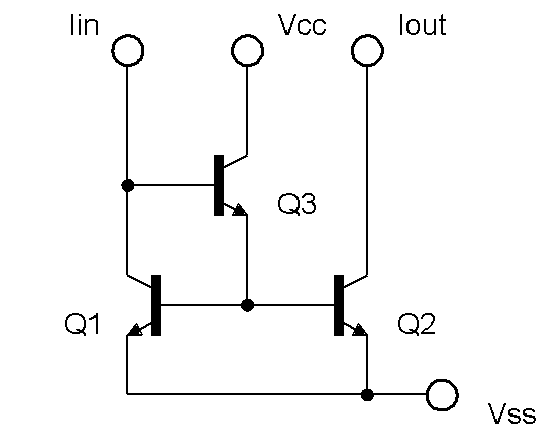
\includegraphics[scale=0.5]{obrazky/ZlepseneWilsonovoZrcadloNPN}
%  \end{center}
%  \caption[Alenčino zrcadlo]{Zlepšené Wilsonovo proudové zrcadlo.}
%\end{figure}
%
%Pro sazbu vektorových obrázků přímo v~\LaTeX{}u je možné doporučit balíček \href{https://www.ctan.org/pkg/pgf}{\texttt{TikZ}}.
%Příklady sazby je možné najít na \href{http://www.texample.net/tikz/examples/}{\TeX{}ample}.
%Pro vyzkoušení je možné použít programy QTikz nebo TikzEdt.
%
%
%
%
%\chapter{Příklad sazby zdrojových kódů}
%
%\section{Balíček \texttt{listings}}
%
%Pro vysázení zdrojových souborů je možné použít balíček \href{https://www.ctan.org/pkg/listings}{\texttt{listings}}.
%Balíček zavádí nové prostředí \texttt{lstlisting} pro sazbu zdrojových kódů, jako například:
%%
%\begin{lstlisting}[language={[LaTeX]TeX}]
%\section{Balíček lstlistings}
%Pro vysázení zdrojových souborů je možné použít
%	balíček \href{https://www.ctan.org/pkg/listings}%
%	{\texttt{listings}}.
%Balíček zavádí nové prostředí \texttt{lstlisting} pro
%	sazbu zdrojových kódů.
%\end{lstlisting}
%%
%Podporuje množství programovacích jazyků.
%Kód k~vysázení může být načítán přímo ze zdrojových souborů.
%Umožňuje vkládat čísla řádků nebo vypisovat jen vybrané úseky kódu.
%Např.:
%
%\noindent
%Zkratky jsou sázeny v~prostředí \texttt{acronym}:
%\label{lst:zkratky}
%\lstinputlisting[language={[LaTeX]TeX},nolol,numbers=left, firstnumber=6, firstline=6,lastline=6]{text/zkratky.tex}
%%
%Šířka textu volitelného parametru \verb|KolikMista| udává šířku prvního sloupce se zkratkami.
%Proto by měla být zadávána nejdelší zkratka nebo symbol.
%Příklad definice zkratky \acs{symfvz} je na výpisu \ref{lst:symfvz}.
%
%\shorthandoff{-}
%\lstinputlisting[language={[LaTeX]TeX},frame=single,caption={Ukázka sazby zkratek},label=lst:symfvz,numbers=left,linerange={bsymfvz-\%\%\%\ esymfvz},includerangemarker=false]{text/zkratky.tex}
%\shorthandon{-}
%
%\noindent
%Ukončení seznamu je provedeno ukončením prostředí:
%\lstinputlisting[language={[LaTeX]TeX},nolol,numbers=left,firstnumber=26,linerange=26]{text/zkratky.tex}
%
%\vspace{\fill}
%
%\noindent
%{\bf Poznámka k~výpisům s~použitím volby jazyka \verb|czech| nebo \verb|slovak|:}\newline
%Pokud Váš zdrojový kód obsahuje znak spojovníku \verb|-|, pak překlad může skončit chybou.
%Ta je způsobená tím, že znak \verb|-| je v~českém nebo slovenském nastavení balíčku \verb|babel| tzv.\ aktivním znakem.
%Přepněte znak \verb|-| na neaktivní příkazem \verb|\shorthandoff{-}| těsně před výpisem a hned za ním jej vraťte na aktivní příkazem \verb|\shorthandon{-}|.
%Podobně jako to je ukázáno ve zdrojovém kódu šablony.
%
%
%\clearpage
%
%%\section{Výpis kódu prostředí Matlab}
%Na výpisu \ref{lst:priklad.vypis.kodu.Matlab} naleznete příklad kódu pro Matlab, na výpisu \ref{lst:priklad.vypis.kodu.C} zase pro jazyk~C.
%
%\lstnewenvironment{matlab}[1][]{%
%\iflanguage{czech}{\shorthandoff{-}}{}%
%\iflanguage{slovak}{\shorthandoff{-}}{}%
%\lstset{language=Matlab,numbers=left,#1}%
%}{%
%\iflanguage{slovak}{\shorthandon{-}}{}%
%\iflanguage{czech}{\shorthandon{-}}{}%
%}
%
%\begin{matlab}[frame=single,float=htbp,caption={Příklad Schur-Cohnova testu stability v~prostředí Matlab.},label=lst:priklad.vypis.kodu.Matlab,numberstyle=\scriptsize, numbersep=7pt]
%%% Priklad testovani stability filtru
%
%% koeficienty polynomu ve jmenovateli
%a = [ 5, 11.2, 5.44, -0.384, -2.3552, -1.2288];
%disp( 'Polynom:'); disp(poly2str( a, 'z'))
%
%disp('Kontrola pomoci korenu polynomu:');
%zx = roots( a);
%if( all( abs( zx) < 1))
%    disp('System je stabilni')
%else
%    disp('System je nestabilni nebo na mezi stability');
%end
%
%disp(' '); disp('Kontrola pomoci Schur-Cohn:');
%ma = zeros( length(a)-1,length(a));
%ma(1,:) = a/a(1);
%for( k = 1:length(a)-2)
%    aa = ma(k,1:end-k+1);
%    bb = fliplr( aa);
%    ma(k+1,1:end-k+1) = (aa-aa(end)*bb)/(1-aa(end)^2);
%end
%
%if( all( abs( diag( ma.'))))
%    disp('System je stabilni')
%else
%    disp('System je nestabilni nebo na mezi stability');
%end
%\end{matlab}
%
%\noindent
%\begin{minipage}{\linewidth}
%
%
%%\section{Výpis kódu jazyka C}
%
%\begin{lstlisting}[frame=single,numbers=right,caption={Příklad implementace první kanonické formy v~jazyce C.},label=lst:priklad.vypis.kodu.C,basicstyle=\ttfamily\small, keywordstyle=\color{black}\bfseries\underbar,]
%// první kanonická forma
%short fxdf2t( short coef[][5], short sample)
%{
%	static int v1[SECTIONS] = {0,0},v2[SECTIONS] = {0,0};
%	int x, y, accu;
%	short k;
%
%	x = sample;
%	for( k = 0; k < SECTIONS; k++){
%		accu = v1[k] >> 1;
%		y = _sadd( accu, _smpy( coef[k][0], x));
%		y = _sshl(y, 1) >> 16;
%
%		accu = v2[k] >> 1;
%		accu = _sadd( accu, _smpy( coef[k][1], x));
%		accu = _sadd( accu, _smpy( coef[k][2], y));
%		v1[k] = _sshl( accu, 1);
%
%		accu = _smpy( coef[k][3], x);
%		accu = _sadd( accu, _smpy( coef[k][4], y));
%		v2[k] = _sshl( accu, 1);
%
%		x = y;
%	}
%	return( y);
%}
%\end{lstlisting}
%\end{minipage}
%
%
%
%
%
%
%
%\chapter{Obsah elektronické přílohy}
%Elektronická příloha je často nedílnou součástí semestrální nebo závěrečné práce.
%Vkládá se do informačního systému VUT v~Brně ve vhodném formátu (ZIP, PDF\,\dots).
%
%Nezapomeňte uvést, co čtenář v~této příloze najde.
%Je vhodné okomentovat obsah každého adresáře, specifikovat, který soubor obsahuje důležitá nastavení, který soubor je určen ke spuštění, uvést nastavení kompilátoru atd.
%Také je dobře napsat, v~jaké verzi software byl kód testován (např.\ Matlab 2018b).
%Pokud bylo cílem práce vytvořit hardwarové zařízení,
%musí elektronická příloha obsahovat veškeré podklady pro výrobu (např.\ soubory s~návrhem DPS v~Eagle).
%
%Pokud je souborů hodně a jsou organizovány ve více složkách, je možné pro výpis adresářové struktury použít balíček \href{https://www.ctan.org/pkg/dirtree}{\texttt{dirtree}}.
%
%\bigskip
%
\chapter{Contents of the Enclosed Electronic Medium}
\label{ch:flash_contents}
{\small
%
\dirtree{%.
.1 /\DTcomment{Root}.
.2 .github\DTcomment{CI workflows and auxiliary files}.
.2 Hardware\DTcomment{Hardware resources for both HW revisions}.
.3 Cube\DTcomment{STM32CubeMX project for pin assigment}.
.3 Docs\DTcomment{Datasheets of components}.
.3 Libs\DTcomment{KiCAD component and footprint libraries}.
.3 rev1\DTcomment{KiCAD project for the first revision}.
.3 rev2\DTcomment{KiCAD project for the second revision}.
.2 Poster\DTcomment{Source file for a future poster}.
.3 poster\_template.pptx.
.2 Software\DTcomment{Software projects and source code}.
.3 controller\DTcomment{The control software}.
.3 embedded\DTcomment{Workspace containing cross-compiled projects}.
.4 firmware\DTcomment{The motor controller's firmware}.
.4 testsuite\DTcomment{Tests for the motor controller's firmware}.
.3 shared\DTcomment{Project with code shared between firmware and controller}.
.3 Cargo.toml\DTcomment{Cargo project file}.
.3 Cargo.lock\DTcomment{Cargo project file lock}.
.3 LICENSE-MIT\DTcomment{Software License}.
.3 README.md\DTcomment{Read me for software}.
.2 Thesis\DTcomment{Source code for this thesis}.
.2 README.md\DTcomment{Readme for this master's project}.
}
}

\chapter{Schematic of the Second Electronics Revision}
\label{ch:rev2_schematic}
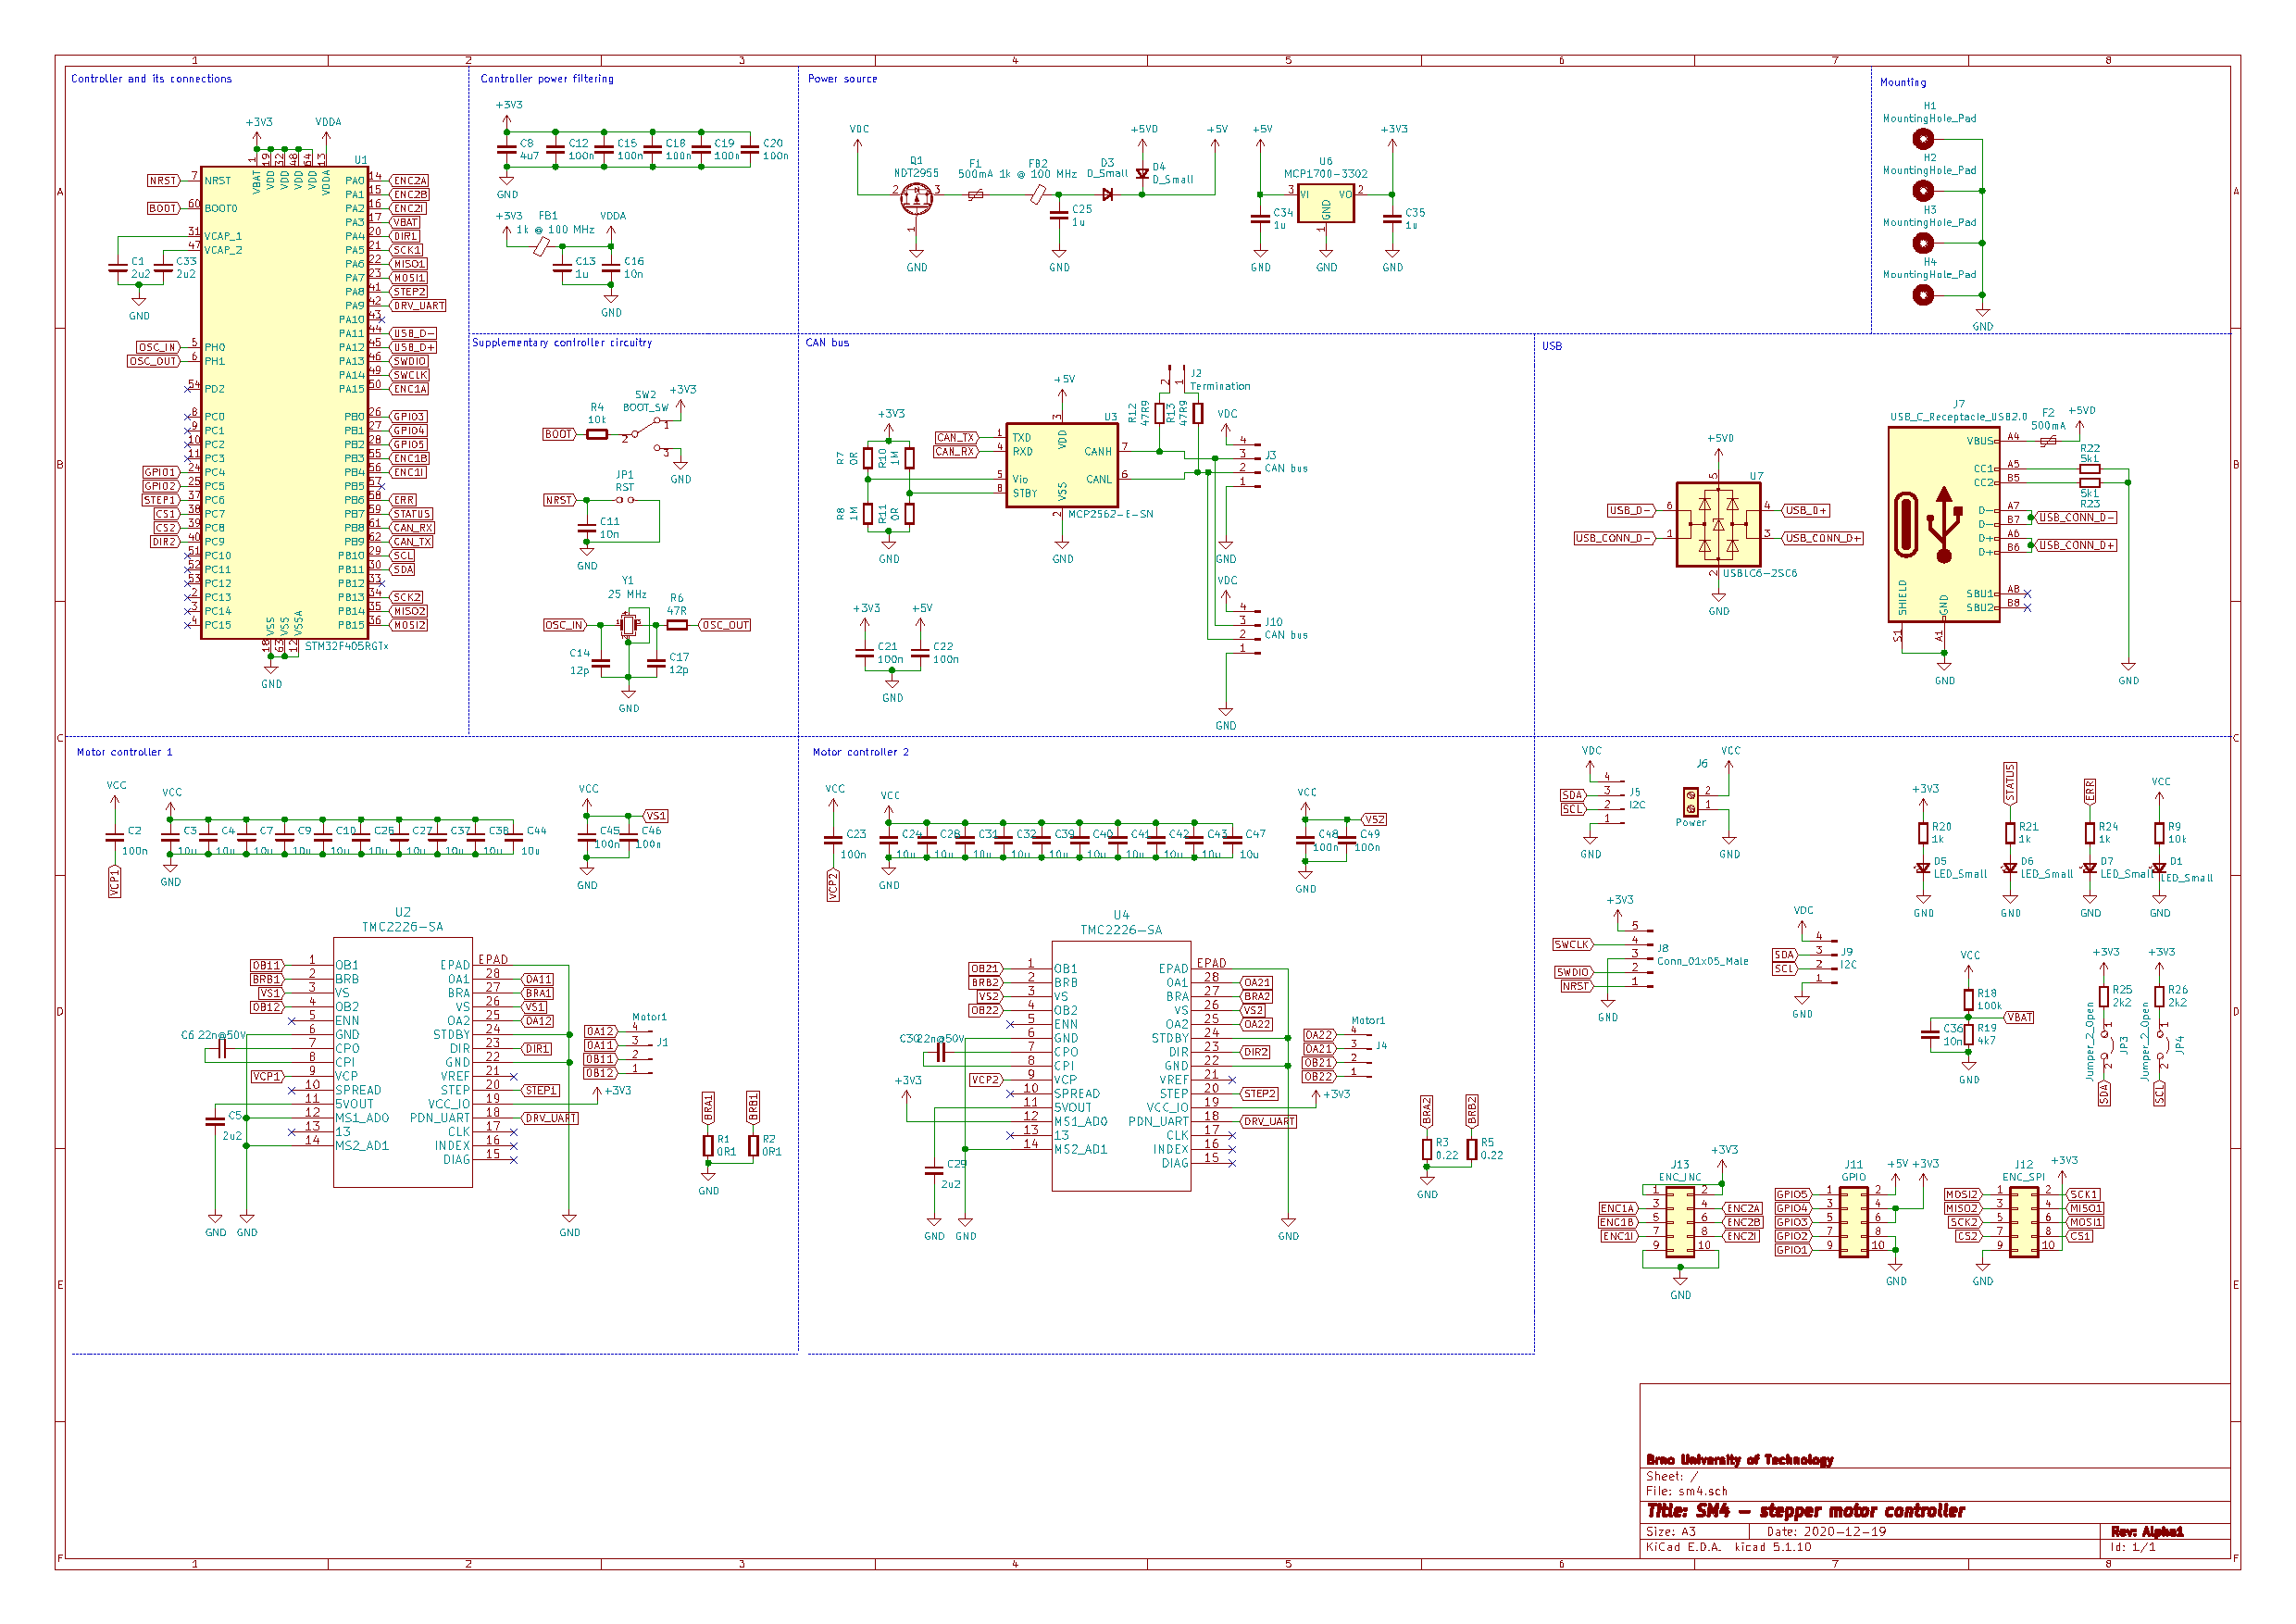
\includepdf[pages=1, landscape=true]{pdf/schematic}

\chapter{PCB of the Second Electronics Revision}
\label{ch:rev2_pcb}
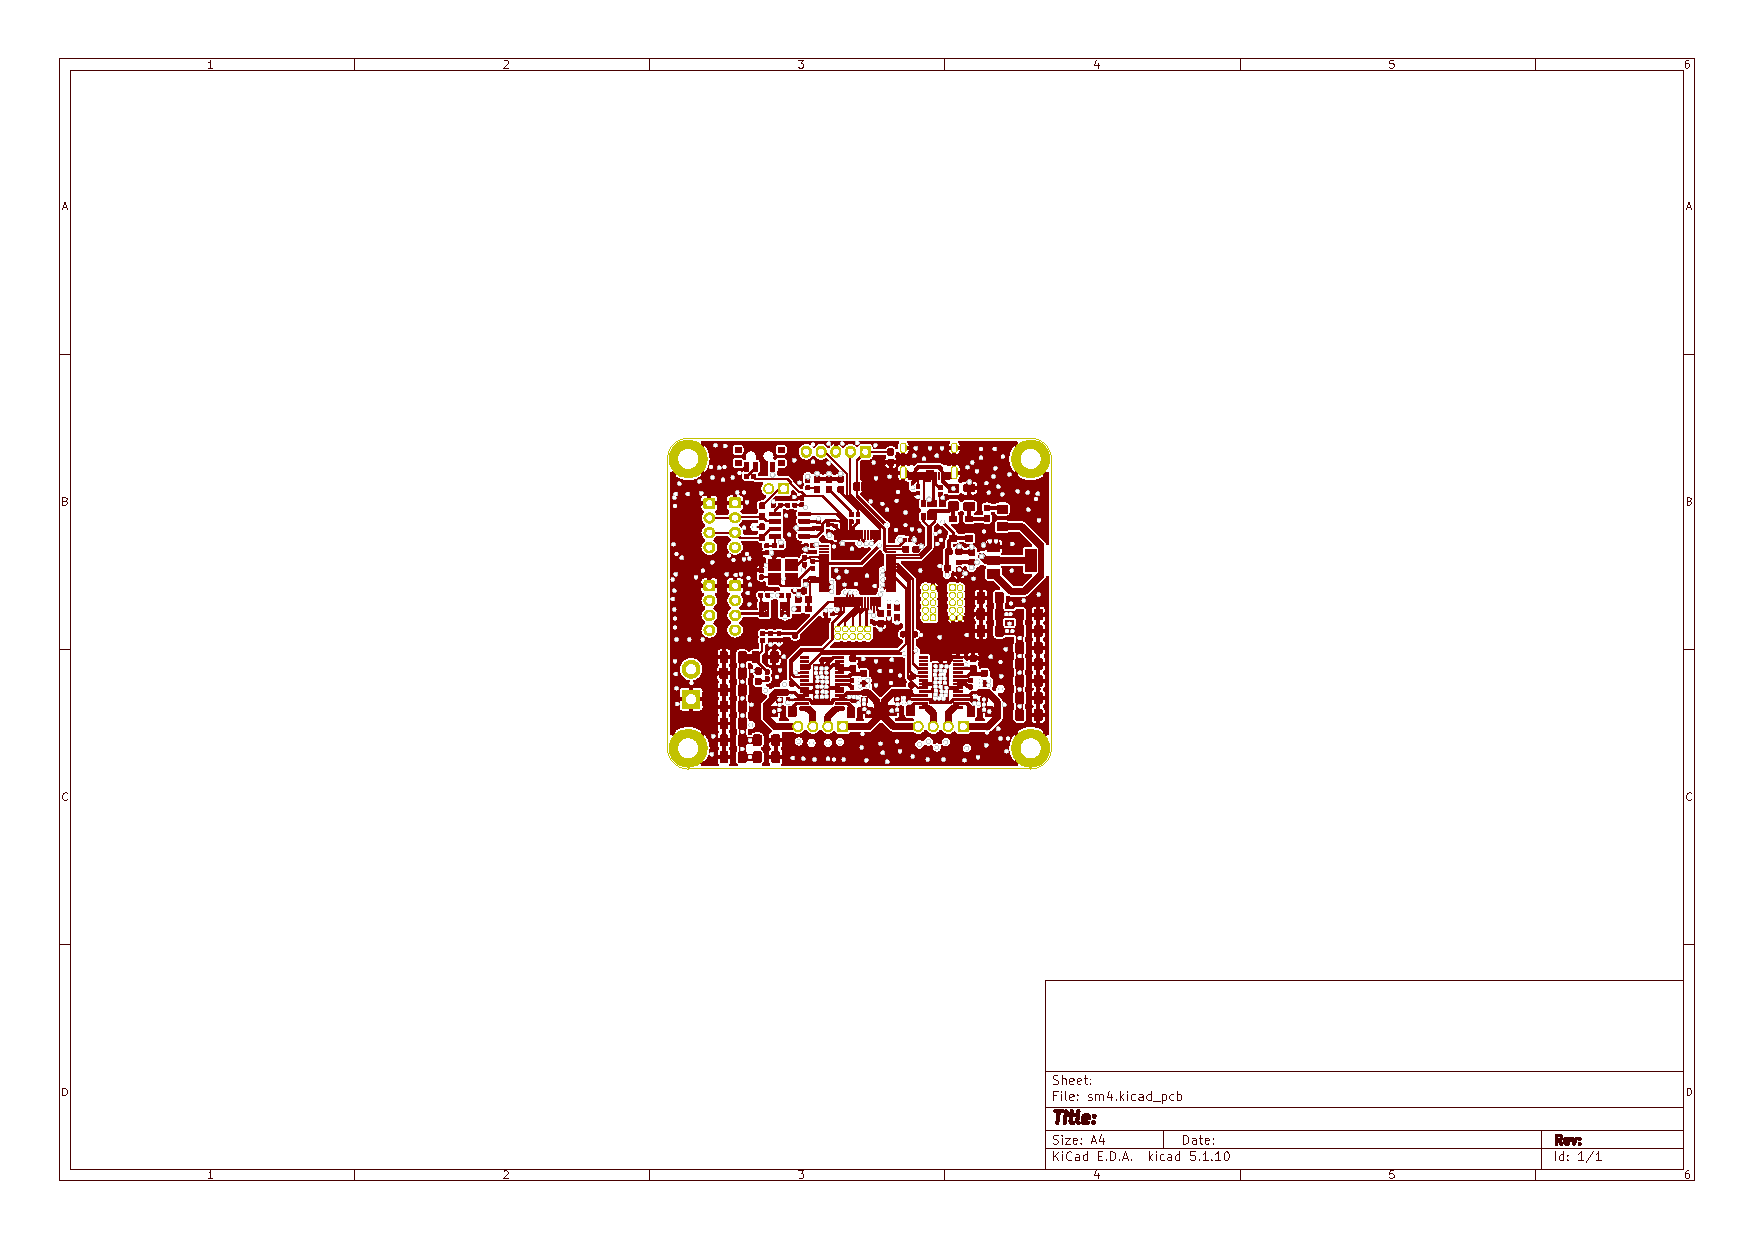
\includepdf[pages=-, landscape=true]{pdf/pcb}

\chapter{CANOpen PDOs and Object Dictionary}
\label{ch:canopen_appendices}
\begin{table}[H]
    \centering
    \begin{tabular}{ |p{1.5cm}|p{1.8cm}|p{1.8cm}|p{2cm}|p{5.5cm}| }
        \hline
        Index & Subindex & Type & Length [B] & Description \\
        \hline
        \hline
        2000 & 1 & f32 & 4 & Battery Voltage in Volts \\
        \hline
        2000 & 2 & f32 & 4 & MCU Temperature in \textdegree C \\
        \hline
        2[1,2]00 & 1 & AxisMode & 1 & mode of the axis - 0 for velocity, 1 for position \\
        \hline
        2[1,2]00 & 2 & bool & 1 & axis enabled \\
        \hline
        2[1,2]00 & 3 & f32 & 4 & target axis velocity in RPS \\
        \hline
        2[1,2]00 & 4 & f32 & 4 & actual axis velocity in RPS \\
        \hline
        2[1,2]00 & 5 & i32 & 4 & target axis position - revolutions \\
        \hline
        2[1,2]00 & 6 & u32 & 4 & target axis position - angle \\
        \hline
        2[1,2]00 & 7 & i32 & 4 & actual axis position - revolutions \\
        \hline
        2[1,2]00 & 8 & u32 & 4 & actual axis position - angle \\
        \hline
        2[1,2]00 & 9 & f32 & 4 & target ramp acceleration in RPS per second \\
        \hline
        2[1,2]00 & 10 & bool & 1 & velocity controller bypass enabled \\
        \hline
        2[1,2]00 & 11 & f32 & 4 & current applied to motor winding during acceleration in Amperes \\
        \hline
        2[1,2]00 & 12 & f32 & 4 & current applied to motor winding when idle in Amperes \\
        \hline
        2[1,2]00 & 13 & f32 & 4 & current applied to motor winding when moving with constant speed in Amperes \\
        \hline
        2[1,2]00 & 14 & f32 & 4 & velocity controller proportional gain \\
        \hline
        2[1,2]00 & 15 & f32 & 4 & velocity controller summation gain \\
        \hline
        2[1,2]00 & 16 & f32 & 4 & velocity controller differential gain \\
        \hline
        2[1,2]00 & 17 & f32 & 4 & velocity controller maximal action value \\
        \hline
    \end{tabular}
    \caption{The Object Dictionary}
    \label{tab:object_dictionary}
\end{table}
\begin{table}[H]
    \centering
    \begin{tabular}{ |p{1.5cm}|p{1.8cm}|p{1.8cm}|p{2cm}|p{5.5cm}| }
        \hline
        Index & Subindex & Type & Length [B] & Description \\
        \hline
        \hline
2[1,2]00 & 18 & f32 & 4 & position controller proportional gain \\
\hline
2[1,2]00 & 19 & f32 & 4 & position controller summation gain \\
\hline
2[1,2]00 & 20 & f32 & 4 & position controller differential gain \\
\hline
2[1,2]00 & 21 & f32 & 4 & position controller maximal action value \\
\hline
\end{tabular}
\caption{The Object Dictionary (Continued)}
\label{tab:object_dictionary2}
\end{table}

\begin{table}[H]
    \centering
    \begin{tabular}{ |p{3cm}|p{2cm}|p{8cm}| }
        \hline
        Value & Length [B] & Description \\
        \hline
        \hline
        axis mode & 1 & LSB contains axis 1 mode - 0 means velocity mode, 1 means position mode, first bit of the second nimble contains axis 2 mode \\
        \hline
        axis enabled & 1 & LSB sets axis 1 enabled - 0 means disabled, 1 means enabled, second lowest bit sets axis 2 enabled \\
        \hline
    \end{tabular}
    \caption{RxPDO1 mapping}
    \label{tab:rxpdo1}
\end{table}

\begin{table}[H]
    \centering
    \begin{tabular}{ |p{3cm}|p{2cm}|p{8cm}| }
        \hline
        Value & Length [B] & Description \\
        \hline
        \hline
        battery voltage & 2 & battery voltage in millivolts \\
        \hline
        temperature & 2 & temperature in tenths of \textdegree C \\
        \hline
    \end{tabular}
    \caption{TxPDO1 mapping}
    \label{tab:txpdo1}
\end{table}


RxPDO2, TxPDO2
\begin{table}[H]
    \centering
    \begin{tabular}{ |p{3cm}|p{2cm}|p{8cm}| }
        \hline
        Value & Length [B] & Description \\
        \hline
        \hline
        axis 1 velocity & 4 & 32-bit float indicating axis 1 velocity in revolutions per second \\
        \hline
        axis 2 velocity & 4 & 32-bit float indicating axis 2 velocity in revolutions per second \\
        \hline
    \end{tabular}
    \caption{Mapping of PDOs containing velocity information - RxPDO2 and TxPDO2}
    \label{tab:velocity_pdo}
\end{table}

\begin{table}[H]
    \centering
    \begin{tabular}{ |p{3cm}|p{2cm}|p{8cm}| }
        \hline
        Value & Length [B] & Description \\
        \hline
        \hline
        axis revolutions & 4 & signed 32-bit integer denoting the number of axis shaft revolutions \\
        \hline
        axis angle & 4 & unsigned 32-bit indicating axis shaft angle \\
        \hline
    \end{tabular}
    \caption{Mapping of PDOs containing position information - RxPDO3, RxPDO4, TxPDO3 and TxPDO4}
    \label{tab:position_pdo}
\end{table}

